Après avoir présenté brièvement les concepts théoriques sur lesquels NODUS se
base, il reste maintenant à analyser les différents coûts qui peuvent être
affectés aux éléments de cette représentation particulière d'un réseau de
transport qu'est le réseau virtuel. Malheureusement, et malgré l'existence de
plusieurs modèles de réseau, la littérature présente très peu de fonctions de
coût concrètes. Tout en présentant et en commentant les éléments de coûts déjà
publiés par ailleurs, les pages qui suivent s'attacheront donc à développer un
cadre méthodologique général et concret, applicable au réseau virtuel.

Les analyses économiques basées sur un modèle de réseau n'ont de sens que si les
poids utilisés pour pondérer les différents arcs du réseau sont crédibles. Ces
poids peuvent être de différentes natures. Il peut s'agir de prix, de coûts, de
temps,... Afin de pouvoir exprimer ces poids de natures différentes en
expression monétaire, on utilise souvent le terme de "coût généralisé", dont une
formulation de base est due à Kresge et Roberts \footnote{Kresge, D.T. et
Roberts, P.O.,1971, "Techniques of Transportation Planning: Systems Analysis and
Simulation Models", Brooking Institution, Washington DC. Une discussion plus
complète sur la définition des composantes d'une fonction de coûts généralisés
est présentée par Wilson A.G. et Bennet R.J., 1985, "Mathematical Methods in
Human Geography and Planning", John Wiley \& Sons, N-Y. } :

$$C_{ij}=f_{ij}+b_1s_{ij}+b_2\sigma s_{ij}+b_3w_{ij}+b_4p_{ij}$$

où:
\begin{itemize}
\item $f_{ij}$: coûts encourus par l'opérateur entre les noeuds i et j
\item $s_{ij}$: temps de voyage entre i et j
\item $\sigma s_{ij}$: variabilité du temps de voyage s
\item $w_{ij}$: temps d'attente avant d'avoir accès au transport
\item $p_{ij}$: probabilité de perte ou de dommage au bien transporté
\end{itemize}


Dans cette formulation, les coefficients $b_n$ qui pondèrent les différentes
compo\-san\-tes de la fonction sont en général proportionnels à la valeur des
marchandises transportées. A l'instar de l'approche de Baumol et Vinod présentée
dans le premier chapitre, le coût généralisé permet d'affecter un coût à tous
les facteurs qui influencent le trafic sur un réseau. Ainsi, un déplacement
exprimé en kilomè\-tres ou un temps d'attente exprimé en heures peuvent tous
deux s'additionner en termes monétaires. Les termes aléatoires repris dans ces
formulations ne peuvent cependant pas être directement affectés au réseau, sauf
s'ils sont intégrés sous forme de moyennes.

Le réseau virtuel nécessite le développement de quatre types de fonctions de
coût. Pour rappel, le type de fonction est déduit de la notation utilisée pour
les noeuds virtuels. Une illustration concrète est présentée dans la table
\ref{tab4_1}.

\begin{itemize}
  \item Déplacement (\textbf{``mv''}): Les identificateurs des noeuds réels sont différents.

  \item Simple passage (\textbf{``tr''}): Les identificateurs des arcs réels sont
différents alors que le mode et le moyen de transport sont restés
identiques.

  \item Transbordement (\textbf{``tp''}): Les identificateurs des arcs réels sont
différents, ainsi que le mode et/ou le moyen de transport.

  \item Chargement (\textbf{``ld''}) / déchargement (\textbf{``ul''}): Un des deux identificateurs
d'arcs réels est "0".
\end{itemize}

\begin{table}[htbp]
\begin{center}
\begin{tabular}{crcccrccc}
\hline

Cas & Noeud1 & Arc1 & Mode1 & Moyen1 & Noeud2 & Arc2 & Mode2 & Moyen2\\
\hline
1 & -1000 & 1000 & 1 & 1 & +1001 & 1000 & 1 & 1\\

2 & +1000 & 1000 & 1 & 1 & -1000 & 1001 & 1 & 1\\

3 & +1000 & 1000 & 1 & 1 & -1000 & 1001 & 1 & 2\\

$4_a$ & -1000 & 0 & 0 & 0 & -1000 & 1001 & 1 & 1\\

$4_b$ & +1000 & 1001 & 1 & 1 & +1000 & 0 & 0 & 0\\
\hline
\end{tabular}
\caption{\label{tab4_1} Codification des ar\^etes virtuelles dans NODUS}
\end{center}
\end{table}

Il reste maintenant à déterminer les éléments de coût qui peuvent être utilisés
dans ces différents cas de figure sachant que dans un premier temps et de
manière intuitive on peut décomposer le coût total de transport de la manière
(comptable) représentée à la figure \ref{f4_1}:

\begin{figure}[htbp]
\centerline{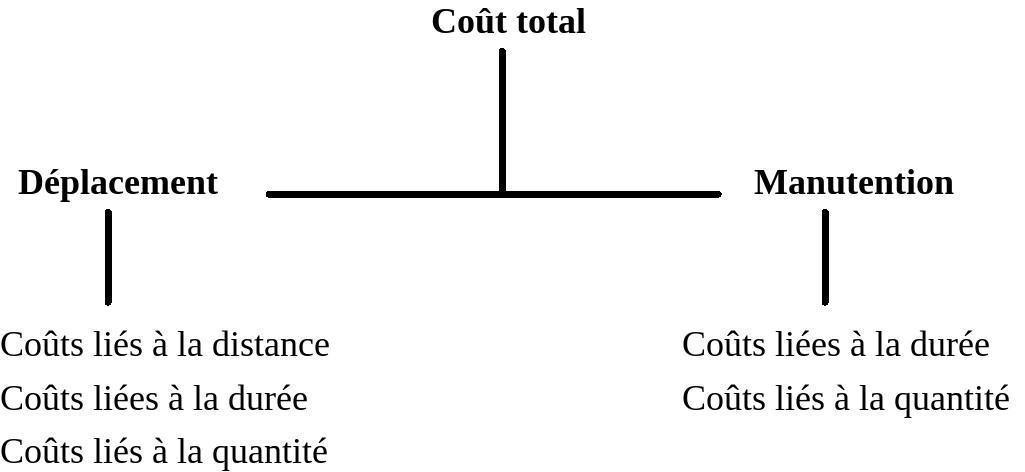
\includegraphics[width=10cm]{f4_1.png}}
\caption{\label{f4_1} Co\^uts de transport}
\end{figure}



\underline{Remarque importante:} Il faut garder à l'esprit que les formes
fonctionnelles qui sont proposées ici ne doivent pas être
considérées comme étant une formulation unique et immuable, mais
plutôt comme une solution bien adaptée à NODUS. Le seul cadre
méthodologique qui est imposé par la notion de réseau virtuel est
qu'il faut développer des fonctions spécifiques pour les quatre cas
énoncés plus haut. La forme fonctionnelle qu'on leur donne est
laissée au libre choix du modélisateur. Ceci étant spécifié, il
peut dès lors être intéressant de donner quelques pistes à suivre,
une sorte de "code de bonne conduite" à respecter dans le
développement de fonctions de coût en environnement multi-modal:

\begin{itemize}
\item Cohérence du point de vue: un transport peut se faire, soit pour
compte propre, soit à l'aide d'un transporteur indépendant. Dans le premier cas,
il faut analyser l'ensemble des coûts supportés par l'entreprise lors du
processus de transport, dans le second cas, c'est la connaissance des tarifs
pratiqués qui est primordiale. Il est donc nécessaire de prendre le même point
de vue pour les différents modes de transport qui sont pris en considération sur
le réseau.

\item Cohérence des unités: lorsqu'une unité de mesure est
choisie (unités moné\-taires par tonne, par kilomètre, par tonne/kilomètre, ...)
pour un mode de trans\-port sur un type d'arc virtuel, il est
évidemment important d'utiliser cette même unité de mesure pour les
autres modes de transport.

\item Cohérence des variables: dans la définition des coûts généralisés,
les mêmes facteurs de coûts doivent être repris pour les différents
modes de transport. Ainsi, si on tient compte de la durée du voyage
ou des coûts financiers pour un mode de transport, ces mêmes coûts
doivent se retrouver dans les fonctions mises au point pour les
autres modes.

\item Cohérence dans le temps: les données utilisées dans les calculs
doivent être compatibles dans le temps (même année de référence)
entre les différents modes de transport .
\end{itemize}

Suite à ces remarques, il est maintenant possible de définir une
approche générale des éléments de coûts applicable à tout problème
traité avec un réseau virtuel.

\begin{itemize}
\item Récolte des données respectant le principe de cohérence dans le
temps.
\item Mise au point des fonctions de coût (respectant les trois
autres principes de cohérence):
        \begin{itemize}
        \item Pour tous les modes et moyens de transport.
        \item Pour les quatre types d'arcs virtuels.
        \end{itemize}
\item Calcul des coûts sur chaque arc virtuel.
\end{itemize}


La littérature propose deux grandes catégories de fonctions de coût. La première
se propose d'analyser l'ensembles des coûts liés aux activités de transport. Il
s'agit d'une démarche de type agrégée qui, par définition, ne s'applique pas à
une utilisation sur un réseau. Par opposition à cette première catégorie, le
second type de fonctions de coût analyse un mouvement d'une origine à une
destination donnée. Malheureusement, ce type de démarche est actuellement
beaucoup moins répandu mais il existe suffisamment de références pour pouvoir se
faire une idée correcte de l'état de l'art en la matière, surtout en ce qui
concerne le transport routier.

Le coût total de transport comprend différents postes qui peuvent
être classés dans les catégories suivantes:

\begin{itemize}
\item Transport proprement dit: tous les coûts inhérents au déplacement
d'un véhicule entre les points d'origine et de destination du
voyage.

\item Valeur d'inventaire: coûts engendrés par la détention de
marchandises durant un certain laps de temps. Ce poste contient des frais réels
tels que les primes d'assurance, des intérêts et un coût d'opportunité (la
marchan\-dise transportée représente une certaine somme d'argent immobilisée, qui
aurait pu être utilisée autrement).

\item Manutention, magasinage: frais inhérents aux manipulations de la
marchan\-dise en dehors du voyage proprement dit. Il s'agit donc
d'emballages, de mise en rayons, de chargements et de
déchargements.

\item Coûts indirects: coûts qui résultent des activités de support à
l'activité de transport (services administratifs,...). Ces coûts ne
sont pas aisément identifiables pour un voyage particulier.
\end{itemize}

En dehors de ces coûts, il faudrait idéalement également prendre en
considération les coûts liées à la congestion et l'impact de la
qualité du transport.

Parmi les autres effets qui influencent le coût du transport se trouve la
congestion. Il paraît évident qu'à un moment où un autre, les usagers d'un
réseau peuvent être confrontés avec des phénomènes de congestion, ce qui doit
être pris en considération lors de l'affectation. Il s'agit donc d'introduire
une méthode qui puisse résoudre les contraintes liées à la capacité du réseau.

Il existe deux manières fondamentalement différentes de procéder
pour tenir compte de la congestion:

\begin{itemize}

\item A un niveau microscopique, la congestion se traduit par un
ralentissement du flux et par un choix de chemins alternatifs pour
éviter les bouchons. La solution à ce problème se trouve dans les
méthodes d'équilibre de réseau qui recalculent les fonctions de
coût au fur et à mesure que le flux augmente. Ces processus
dynamiques prennent explicitement en consi\-dération des contraintes
comme la capacité des voies ou la congestion au niveau des
terminaux.

\item A un niveau macroscopique, il n'est pas toujours important de
savoir que tel ou tel carrefour est saturé à 8 heures du matin,
dans la mesure où ce carrefour n'est même pas repris dans le
réseau. Par contre, il faut tenir compte de considérations
générales telles que la traversée de grandes villes ou l'attente à
certaines frontières. Ce point de vue macroscopique affecte les
fonctions de coût, mais pas forcément les chemins utilisés. En
effet, lorsque l'on digitalise un grand réseau tel que le réseau
des axes de communication d'intérêt international européen, on ne
s'occupe que très rarement  du détail de ce qui se passe dans une
ville. Dans un tel  cas, un arc digitalisé peut même représenter
plusieurs routes plus ou moins parallèles qui se répartiront le
trafic. Le coût de la congestion macroscopique peut alors tout
naturellement être imputé à des arcs virtuels de type "simple
passage", sous forme d'un coût (fixe) par heure perdue .
\end{itemize}


La qualité du transport est à prendre dans un sens très large et
elle représente essentiellement la dimension multi-produits du
processus de transport. En effet, la distinction entre les
différents produits n'a pour l'instant pas encore été faite, sauf
en ce qui concerne leur valeur d'inventaire. Mais cette valeur
n'est pas représentative, dans la mesure où des moyens de transport
différents peuvent être utilisés pour transporter des marchandises
de catégories différentes. On peut imaginer deux marchandises, dont
la valeur à la tonne est comparable, qui pourraient être
transportées par les même modes de transport, mais qui, dans la
pratique, sont transportées par des modes de transport différents,
avec des coûts différents. Le choix du mode de transport est donc
également influencé par une certaine qualité de ce transport, qui
est difficilement traduisible en termes monétaires.

Prenons l'exemple d'un fabricant belge de vêtements qui exporte
vers la France. Il choisit d'effectuer le transport par camion,
alors que le train serait moins cher. Mais le camion offre pour lui
deux avantages:
\begin{itemize}
\item Il peut effectuer un transport de porte à porte
\item Il transporte les pièces vestimentaires sur des cintres pendus dans
le camion. De cette manière, la marchandise ne se chiffonne pas et
garde toute sa valeur.
\end{itemize}
Quelle est la valeur à attribuer au fait qu'un vêtement ne se
chiffonne pas?

Bien que des facteurs comme le temps, la fréquence ou la fiabilité
soient souvent présents, le concept de qualité n'est pas facile à
introduire dans une fonction de coût. De plus, il n'est pas facile
de savoir à quel moment la qualité joue un rôle. Est-ce lors du
chargement ou du déplacement? Cette discussion dépasse le
cadre de cette courte note méthodologique.

En partant de la définition du réseau virtuel qui nécessite quatre types de
fonctions de coût, le tableau \ref{tab4_2} résume assez bien les types de coûts
qu'il est bon de prendre en considération:

\begin{table}[htbp]
\begin{center}
\begin{tabular}{ll}
\hline

Type d'arc virtuel  &Nature des coûts\\
\hline
Déplacement         & Transport\\
                    & Valeur d'inventaire\\
                    & Coûts indirects\\

Transbordement      & Manutention\\
                    & Valeur d'inventaire\\
                    & Coûts indirects\\

Chargement et Déchargement & Manutention\\
                           & Magasinage\\
                           & Valeur d'inventaire\\
                           & Coûts indirects\\

Simple passage             & Congestion au sens large\\
\hline
\end{tabular}
\caption{\label{tab4_2} Types de co\^uts sur les arcs virtuels}
\end{center}
\end{table}












